% !TEX TS-program = pdflatex
% !TEX encoding = UTF-8

\documentclass[a4paper,11pt,twoside,english]{toptesi}
\usepackage[latin1]{inputenc}
\usepackage[T1]{fontenc}
\usepackage{lmodern}
\usepackage[a-1b]{pdfx}
\usepackage{hyperref}
\usepackage{cite}
\usepackage{listings}
\usepackage{color}
\usepackage{url}
\usepackage{multirow}
\usepackage{amsmath}
\usepackage{verbatim}
\usepackage{tikz}
\usepackage{rotating}
\usepackage{booktabs}
\usepackage{float}
\usetikzlibrary{arrows.meta,positioning,calc}

% Definition of a new language for listings
%\lstdefinelanguage{P4}
%{
%	% list of keywords
%	alsoletter=\#,
%	morekeywords={
%		header\_type,
%		fields,
%		header,
%		parser,f
%		extract,
%		return,
%		default,
%		next,
%		\#define,
%		latest,
%		select,
%		apply,
%		control,
%		table,
%		reads,
%		actions,
%		modify\_field,
%		action,
%		valid,
%		nop,
%		exact,
%		lpm,
%		if,
%		hit,
%		and,
%		extern,
%		void,
%		bit
%	},
%	sensitive=true, % keywords are not case-sensitive
%	morecomment=[l]{//}, % l is for line comment
%	morecomment=[s]{/*}{*/}, % s is for start and end delimiter
%	morestring=[b]" % defines that strings are enclosed in double quotes
%}
%
%\definecolor{eclipseBlue}{RGB}{42,0.0,255}
%\definecolor{eclipseGreen}{RGB}{63,127,95}
%\definecolor{eclipsePurple}{RGB}{127,0,85}
%
%\lstset{
%	language={P4},
%	basicstyle=\fontsize{8}{9}\ttfamily, % Global Code Style
%	captionpos=b, % Position of the Caption (t for top, b for bottom)
%	extendedchars=true, % Allows 256 instead of 128 ASCII characters
%	tabsize=2, % number of spaces indented when discovering a tab 
%	columns=fixed, % make all characters equal width
%	keepspaces=true, % does not ignore spaces to fit width, convert tabs to spaces
%	showstringspaces=false, % lets spaces in strings appear as real spaces
%	breaklines=true, % wrap lines if they don't fit
%	frame=trbl, % draw a frame at the top, right, left and bottom of the listing
%	%frameround=tttt, % make the frame round at all four corners
%	framesep=4pt, % quarter circle size of the round corners
%	numbers=left, % show line numbers at the left
%	numberstyle=\tiny\ttfamily, % style of the line numbers
%	commentstyle=\color{eclipseGreen}, % style of comments
%	keywordstyle=\color{eclipsePurple}, % style of keywords
%	stringstyle=\color{eclipseBlue}, % style of strings
%}

\hypersetup{%
    pdfpagemode={UseOutlines},
    bookmarksopen,
    pdfstartview={FitH},
    colorlinks,
    linkcolor={blue},
    citecolor={blue},
    urlcolor={blue}
  }

\newtheorem{osservazione}{Osservazione}% Standard LaTeX
\newtheorem{definition}{Definition}


\begin{document}
\english

\ateneo{Politecnico di Torino}
\corsodilaurea{Computer Engineering}

\titolo{Exploring the effectiveness of number formats in GPU-accelerated programs}

\candidato{Giovanni \textsc{Santangelo}}
\relatore{Prof.\ Esteban \textsc{Rodriguez Condia}}
\secondorelatore{Prof.\ Matteo \textsc{Sonza Reorda}}
\terzorelatore{Prof. \ Juan David \textsc{Guerrero Balaguera}}
\sedutadilaurea{\textsc{Academic~Year} 2025-2026}
\logosede{Cover/Logoblu}

\CorsoDiLaureaIn{Master Degree course in\space}
\TesiDiLaurea{Master Degree Thesis}
\InName{in}
\CandidateName{Candidate}
\AdvisorName{Supervisors}


\frontespizio % make cover page

\ringraziamenti

Write here you acknowledgments. 

\abstract
In recent years, Graphics Processing Units (GPUs) and specialized hardware accelerators have become central to high-performance computing, particularly for deep learning and matrix-intensive workloads. A significant part of their efficiency comes from dedicated compute units that accelerate dot-product and multiply-accumulate operations using reduced-precision and format-specific arithmetic. While floating-point and integer representations remain widely used, alternative numerical formats such as lower precisiom floating-points and fixed-point, posit, and logarithmic number system representations are increasingly considered as possible solutions for improving efficiency, accuracy, or robustness. However, the architectural implications of supporting these formats inside tensor-core-like accelerator datapaths require further investigation.

This thesis investigates the design, validation, and integration of configurable arithmetic architectures for matrix-oriented acceleration. The work first develops a parametric Dot Product Unit (DPU) supporting multiple numerical representations, including integer, fixed-point, floating-point, posit, and logarithmic formats. Each format-specific datapath implements the same dot-product computational model, allowing the behavior of different arithmetic representations to be compared under a common functional structure. The individual datapaths are developed at RTL level and validated through simulation-based testbenches against golden reference results.

Starting from the parametric DPU, the work extends the design toward a higher-level Tensor Core Unit (TCU) architecture intended to support matrix-oriented operations. The proposed accelerator is then considered in two different integration contexts: a GPU-like environment based on FlexGrip Plus and a RISC-V-based environment based on the PULPino-Klessydra core. These integration paths require dedicated control logic, operand handling, custom instruction support, and result writeback mechanisms.

The thesis evaluates the proposed architectures in terms of functional correctness, hardware resource utilization, numerical behavior, and resilience-related considerations. Overall, the work aims to clarify the trade-offs between numerical format choice, architectural complexity, and computational robustness, contributing to the study of future hardware accelerators supporting emerging number formats.

\indici

\mainmatter

% !TEX root = ../main.tex

\chapter{Introduction}


In this chapter, you must provide an overview of your thesis, written such that a non-engineer person (one of your parents) should be able to read and understand at high level.
\begin{itemize}

\item what is you main contribution? 
\item which methodology you used? (theory, simulation, experiments, literature overview)?
\item how the thesis is organized? which topic is covered in each chapter?

 \end{itemize}


\section{Motivation and Context}

Artificial Intelligence (AI) has become increasingly important in modern
computing systems worldwide, ranging from everyday applications such as
conversational assistants and recommendation systems to more complex tasks
involving prediction, classification, perception, autonomous decision-making,
and many others. Many of these applications rely on machine learning models
whose execution requires a large number of numerical operations. In particular,
Deep Neural Networks (DNNs) and other AI models are largely based on repeated
dot products and matrix multiply-accumulate operations, which represent
fundamental computational kernels in several AI workloads.

For this reason, the design of hardware architectures capable of accelerating
these mathematical operations has become a relevant topic in both academic and
industrial research. Specialized hardware accelerators can improve the execution
of matrix-based computations by exploiting parallelism and by using internal
arithmetic units optimized for specific numerical formats. This is especially
important because the efficiency of AI execution does not depend solely on the
algorithm itself, but also on how the underlying hardware represents, moves, and
processes the numerical data.

Therefore, the choice of the numerical format used during the execution of a
given AI model directly affects several important design aspects of the
associated accelerator circuit, including performance, circuit area, energy
efficiency, numerical accuracy, and resilience to faults. These aspects motivate
the study of hardware architectures capable of supporting and comparing multiple
numerical formats within the same computational framework.


\section{Problem Statement}

As mentioned previously, the problem addressed in this thesis concerns the
efficient design of dedicated accelerators for the numerous matrix
multiply-accumulate (MMA) operations involved in AI and DNN workloads.
Moreover, such calculations are performed by accelerators through the encoding
of the matrix elements into a specific numerical format. Depending on the
selected format, the hardware architecture of the accelerator determines how
data is computed, stored, moved, and approximated. Therefore, the choice of
the numerical format used during the execution of a given workload affects
both the hardware design of the accelerator and its related metrics.

At present, conventional standard formats such as half-precision and
single-precision floating-point, as well as integer representations, are
widely used in today's accelerators embedded in Graphics Processing Units
(GPUs), Central Processing Units (CPUs), and other hardware platforms. At the
same time, emerging number formats such as posit, fixed-point, logarithmic,
and reduced-size floating-point and integer formats also exist. However, their
usefulness is not always obvious until appropriate accelerators involving
their use are implemented, integrated, and tested.

Consequently, the problem grows in scope when the availability of multiple
possible numerical formats is taken into account. This thesis addresses this
problem through the design, integration, and testing, using hardware
description tools, of a configurable acceleration architecture based on a
Tensor Core Unit (TCU) composed of multiple Dot Product Units (DPUs). The goal
is to support matrix-oriented computations through different numerical formats
and to enable their comparison in terms of correctness, performance, hardware
cost, numerical behavior, and resilience to faults.

\section{Thesis Objectives}

The main objective of this thesis is to investigate the role of different
numerical formats in hardware accelerators for matrix-oriented computations.
The work aims to study how conventional and emerging number formats can be
supported at hardware level and how their use affects the design of
accelerator architectures.

More specifically, the thesis aims to define a configurable acceleration
architecture for multiply-accumulate operations, integrate it into
representative GPU-like and processor-based environments, and validate its
behavior through simulation and comparison with reference results.


\section{Main Contributions}

Following the mentioned objectives, the main contributions of this thesis can be summarized as follows:

\begin{itemize}

\item A configurable RTL-level Dot Product Unit architecture for
matrix-oriented multiply-accumulate operations under different numerical
formats.

\item A parametric Tensor Core Unit architecture composed of multiple Dot
Product Units and the required control, operand handling, and result
management logic.

\item The integration of the proposed Tensor Core Unit into two different
hardware contexts: the FlexGrip Plus GPU-like architecture and the
PULPino-Klessydra RISC-V core.

\item A functional validation flow based on simulation and comparison with
golden/reference results for verifying the correct behavior of the integrated
accelerator.

\item A hardware-oriented framework that provides a basis for the study of different
numerical formats in terms of correctness, performance, hardware cost,
numerical behavior, and resilience to faults.

\end{itemize}



\begin{itemize}
\item what is the addressed scenario and the addressed problem?
\item why the problem you addressed is interesting and/or practical relevant?

\end{itemize}
Why Number Formats Matter in Hardware Accelerators 


\section{Main Contributions}
\section{Thesis Organization}


\chapter{Background and Related Work}

\section{Matrix-Based Computation in AI Workloads}
%purpose of the section: Explain why AI/DNN workloads become matrix-based workloads

%Goal of this section:
%
%Explain why modern AI and DNN workloads are strongly based on matrix, vector and tensor computations. This section should prepare the reader for the next section on dot product and multiply-accumulate operations.
%
%Paragraph1:
%
% What kind of numerical objects are used in neural networks ?
% Mention inputs, weights, activations, and outputs.
% Explain that they are commonly represented as vectors, matrices, or tensors.
% Do not discuss hardware details.
%
Neural networks operate on numerical data that is usually organized in the
form of vectors, matrices, or tensors. Inputs, weights, intermediate
activations, and outputs of a layer of a neural network can all be represented with these structures. This
makes many neural network computations strongly related to linear algebra,
because the same type of arithmetic operation is repeated many times over
large groups of values. For this reason, matrix-based computation is one of
the main computational patterns involved in modern AI workloads.

%Paragraph 2:
% Why do neural network layers involve linear algebra ?
% Explain that many layers compute weighted combinations of input values.
% Mention that this naturally leads to matrix-vector or matrix-matrix operations. 
%
Neural networks are composed of many layers, each computing its outputs from the previous layer's values. Specifically, each layer contains an interconnection of neurons, which form combinations of values to pass to the subsequent layers. Each neuron performs this operation by multiplying the input values by its learned weights. After these multiplications, the products computed by the neurons are summed together along with a bias. Therefore, in the layers of a neural network, there are groups of mathematical operations equivalent to a dot product plus bias. Specifically, one dot product operation is associated with the workload of a neuron, but since layers contain groups of neurons, the layer performs many dot product operations collectively. As a consequence, these many dot products can be grouped together mathematically as a matrix-vector multiplication; when multiple input samples are processed together as a batch, this becomes a matrix-matrix multiplication. For this reason, neural network layers are strongly connected to linear algebra operations \cite{higham2018deeplearning}.

%Paragraph 3:

% Where do matrix operations appear in actual DNN models ?
% Mention fully connected layers and batched execution 
% Mention that convolutional layers can also be implemented through matrix-based kernels such as GEMM-style approaches
% Possible citation: \cite{anderson2017lowmemory}

The matrix-based computations previously introduced appear in specific
layers of a typical deep neural network. Since a deep neural network
contains different types of layers, the amount of matrix-based computation
depends on the layer type. Typically, fully connected layers and
convolutional layers contain large numbers of matrix-based operations
\cite{higham2018deeplearning}. In fact, even though convolutional layers
are spatial/filter operations, they are often implemented or reorganized
through matrix-based kernels. It is common for the operations performed by
convolutional layers to transform the mathematical convolution into
general matrix multiplication (GEMM), allowing the same computation to be
performed through optimized matrix multiplication routines
\cite{anderson2017lowmemory}. Therefore, since these layers are commonly found in deep neural networks, matrix multiplication appears repeatedly in DNN
training and inference.

%Paragraph 4:

% Why are these operations computationally important ?
% Explain that DNN training and inference repeat these operations many times over large numbers of parameters and activations.
% Possible citation: \cite{sze2017efficient}
Matrix-based operations are computationally important in DNNs because they are repeatedly executed across many layers. Modern neural networks contain many activations and parameters during both inference and training. During inference, the network performs a forward pass through the layers to produce an output. During training, the cost is higher because the model also performs backpropagation and updates the weights used by each layer. These computations are applied to large tensors, so the total number of arithmetic operations becomes very high. Therefore, matrix-based computation represents a major part of the DNN workload and one of the dominant sources of computational cost \cite{sze2017efficient}.

%Paragraph 5:

% Why does the computational cost of DNNs motivate hardware acceleration ?
% Explain that when the dominant computation is regular and matrix-based, specialized hardware can exploit parallelism and repeated arithmetic patterns.
% Possible citation: \cite{chetlur2014cudnn}
Since matrix-based operations represent a major part of DNN workloads, they are natural candidates for acceleration. Their structure is regular and repetitive, because similar arithmetic patterns are applied over many tensor elements. This regularity exposes data-level parallelism. For this reason, GPUs and specialized accelerators can be useful, as they exploit parallelism by executing many arithmetic operations concurrently \cite{sze2017efficient}. For instance, this is also why optimized libraries such as cuDNN provide efficient implementations of common DNN primitives \cite{chetlur2014cudnn}. Consequently, studying dedicated hardware units for matrix, dot-product, and MAC acceleration is well motivated.
%Paragraph 6:

% Transition to the next section
% Explain that matrix multiplication is ultimatly decomposed into dot products and multiply accumulate operations, which are the arithmetic kernels studied in the next section.
DNN workloads are often described at the matrix level. Each element of an output matrix is computed from a row of one matrix and a column of another matrix. And this specific row-column calculation correspond to a dot-product operation, which is formed of repeated products and accumulations of such products. In the industry, the operation of a multiplication between two values and the addition of a third is known as Multiply and Accumulate (MAC). The next section focuses on dot product operations and MAC operations specifically, as  they are the basic kernels behind matrix multiplication acceleration.


\section{Dot Product and Multiply-Accumulate Operations}

\section{Tensor Core Units and HMMA-style Execution}

\section{Numerical Formats in Hardware}

\section{GPU Architecture and the FlexGrip Plus}
Here I will answer these questions: what are gpus and describe how they have increased in popularity in today's period of machine learning and artificial intelligence

\section{RISC-V Architecture and the Klessydra T13}

\section{Fault Resilience and Fault Injection in Hardware Accelerators}

\section{Related Work}


\chapter{Parametric Dot Product Unit Architecture}
\label{ch:parametric_dpu}
%in this chapter i talk about the first real contribution chapter. Chapter 2 explained the background, chapter 3 explains what architecture i have designed and compared....

%chapter 3 will be about design description of the dpus for the formats + the construction + the validation flow... the error graphs and performance reports dont need to be showed in this chapter, those will be moved mostly to the evaluation chapter.

%chapter 3 explains what i have built and how i have built it in the sense of the DPUs.

\section{Chapter Overview}

The previous chapter introduced the general concepts needed to understand matrix-based computation, dot product operations, along with the general information of the GPU and RISC-V like architectures which the final parametric accelerator is meant to live. Starting from those concepts this chapter focuses on the first level of design and validation of the Parametric Dot Product Unit (DPU). The objective is to describe the approach of how the different numerical-format datapaths were constructed, individually verified, and then integrated into a common top level architecture.

The proposed architecture is based on a dot-product computation that combines multiple multiplication operations with accumulation stage. This operation is representative of the arithmetic pattern used in matrix multiplication and neural network workloads as described previously. For this reason, the DPU is used as a basic computational block for comparing different numerical formats under the same functional model. 

The design process of this first release of the parametric DPU followed a format-specific approach; First, dedicated DPUs were constructed for each numerical rapresentation considered in the thesis, including floating-point, integer, fixed-point, posit, and logarithimn number systems formats. After this standalone validation phase, the individual datapaths of the separate DPUs were integrated into a top-level wrapper, where the selected numerical format and operand width determine which internal DPU is used for the computation at hand.

\section{Dot Product Computational Model}

Generally, given a format, the DPU considered in this thesis computes a fixed-size multiply-accumulate operation based on four pairs of input operands and one additional accumulation input. More specifically, the unit receives four operands from a first input vector, four operand from a second one, and an additional scalar value which is accumulated. Equation ~\eqref{eq:dpu_computational_model} depicts this concepts more clearly. In the equation, $A_i$ and $B_i$ represent the input operand pairs, $C_0$ represents the initial accumulation value, and $R$ is the final result produced by the DPU. This operation corresponds to a small dot-product computation with an additional accumulation term, making it compatible with the multiply-accumulate structure discussed in Chapter~\ref{ch:background}.

\begin{equation}
R = A_0B_0 + A_1B_1 + A_2B_2 + A_3B_3 + C_0
\label{eq:dpu_computational_model}
\end{equation}

The choice of a four-product structure is motivated by the fine-grained organization of Tensor Core-like matrix multiply-accumulate operations. As discussed in the previous chapter, Tensor Core execution can be viewed as a matrix-level operation decomposed into smaller dot-product computations. In particular, a 4-by-4 matrix multiply-accumulate operation can be decomposed into sixteen four-element dot products \cite{raihan2019modeling}. For this reason, the DPU adopted in this work is organized as a four-lane dot-product block with an additional accumulation input. The term $C_0$ represents the incoming accumulation value, while the four products $A_iB_i$ represent the four multiplicative contributions of a reduced dot-product operation.

The same computational model describes is adopted for all the DPU variants considered in this thesis. This choice make it possible to compare different numerical formats under the same operation, while changing only the arithmetic representation and the internal datapath used to compute the result. Therefore, the floating-point, integer, fixed-point, posit, and LNS implementations all target the same mathematical behavior, but they differ in the way multiplication, accumulation, rounding, scaling, and special cases are handled internally.

This common computational model is important because it separates the functional objective of the DPU from the implementation details of each numerical format. The following sections therefore describe how the same dot-product operation was implemented through different format-specific datapaths and how each variant was validated before being integrated into the top-level parametric architecture.

\section{Format-Specific DPU Construction}

%section which explains my real construction flow.... in the sense that i didnt immediatly build one magic parametric DPU immediatly, but i have built one specific DPU per format first !
The construction of the first release of the parametric DPU started from the development of individual format-specified DPU variants. Instead of immediatly designing a single unified datapath for all the formats, for this first release each numerical rapresentation was first treated independently.This approach made it possible to focus on the arithmetic requirements of each format and to validate the corresponding datapath in isolation before integrating it into the final parametric architecture.

Althoguh all variants implement the same computational model, the internal datapath organization is not nessarily identical for every format for this first release. As introduced in Section~\ref{sec:dpus_structures}, the general dot-product operation can be organized either through an early-accumulation structure or through a multiplier-and-adder-tree structure.Depending on the arithmetic operators available in the FloPoCo library for a given representation, the DPU was constructed either by a chain of multiply accumulate stages or by combining separate multiplier and adder blocks.

\subsection{Arithmetic Operator Generation with FloPoCo}
All the arithmetic operators used for the formats were generated using FloPoCo. FloPoCo is an arithmetic core generator that produces hardware descritpion of numerical operators with particular ephasis on Field Programmable Gate Array (FPGA)- oriented arithmetic datapaths \cite{dedinechin2011flopoco}. In this work, it was used to generate parametrized arithmetic components by specifying the numerical format parameters required by each implementation.
For the floating-point variants, FloPoCo allowed the exponent and fraction widths to be selected according to the target precision. This made it possible to generate operators for reduced-precision arithmetic which involved 8 bit operand, as well as generating more common circuits supporting more bits in their operands. The generated components were then manually interconnected to construct complete DPU variants implementing the computational model defined in Equation~\eqref{eq:dpu_computational_model}.

\subsection{Floating-Point DPU Variants}
%subsection should explain: that i started from floating point format, that i used flocopoco to generate arithmetic operators. for Fp16 I generated/used MAC or multiplier adder blocks. I manually interconnected the generated blocks. The result was a format-specific FP16 DPU computing the same equation. Later the same approach was repeated for other floating point widths operands.

The first family of format-specific datapaths developed in this work is based on the floating-point arithmatic. For this type of format, three DPU variants were considered each constructed considering the widths of the operands as 8 bits, 16 bits, and 32 bits respectively. These variants are refered to as FP8E4M3,  FP16, and FP32 in the rest of the thesis. FP8E4M3 rapresents a reduced-precision floating point format, while FP16 and FP32 correspond to half-precision floating-point arithmetic, respectively. 

Following the FloPoCo-based generation approach described above, the arithmetic operators for each floating-point width were generated by selecting the appropriate exponent and fraction parameters. The generated operators were then interconnected to implement the four-product accumulation structure of the DPU. In this way, each floating-point variant computes the same mathematical operation, while using arithmetic components configured for the target precision.

The floating-point DPU variants were implemented using an early-accumulation structure based on a chain composed of four multiply and accumulate circuits. Each MAC circuit component had been generated thorugh FloPoCo as discussed. Each MAC stage then multiplies one pair of operands and adds the result to the partial sum produced by the previous MAC. After the four MAC stages, the final output corresponds to the complete dot-product result.

This organization was adopted for the floating-point datapaths because configurable floating-point MAC operators were available through FloPoCo. As a result, the FP8E4M3, FP16, and FP32 DPUs share the same early-accumulation structure, while differing in the numerical precision and in the internal parameters of the generated arithmetic operators.

\subsection{Integer DPU Variants}

The integer DPU variants were developed to evaluate the behavior of the dot-product architecture when using fixed-width integer arithmetic. Two integer configurations were considered in this work: \texttt{INT8\_16} and \texttt{INT16\_32}. In the first case, the input operands are represented using 8-bit integer values, while the internal accumulation and output are represented on 16 bits. In the second case, the input operands use 16-bit integer values, while the accumulation and output are represented on 32 bits. This choice allows the result of the multiplications and additions to be represented with a wider word length than the input operands, reducing the risk of overflow during the accumulation stage.

Unlike the floating-point DPU variants, the integer datapaths were implemented using a multiplier-and-adder-tree organization. In this structure, the four products $A_iB_i$ are computed first by four parallel integer multipliers. The resulting products are then combined through a tree of adders, together with the accumulation input $C_0$, to produce the final output $R$. This organization directly reflects the dot-product equation introduced in Equation~\eqref{eq:dpu_computational_model}.

The use of a multiplier-and-adder-tree structure was suitable for the integer variants because the required arithmetic operators are simpler than exponent-based formats and can be directly implemented using fixed-width multipliers and adders. Therefore, the \texttt{INT8\_16} and \texttt{INT16\_32} DPUs preserve the same functional behavior as the floating-point variants, but use a different internal datapath organization based on parallel product generation followed by tree-based accumulation.

\subsection{Fixed-Point DPU Variants}
%paragraph1: to explain what fixed-point variants exist in my design
The fixed-point DPU variants were developed to evaluate dot-product computation using fixed-width arithmetic with an implicit scaling factor. Similarly to the integer related DPUs, two fixed-point configurations were considered in this work: \texttt{FXP8\_16} and \texttt{FXP16\_32}. In these configurations, the first number indicates the input operand width, while the second number indicates the wider accumulation and output width. This organization allows the products and partial sums to be represented with a larger word length than the input operands.
%paragraph 2: specifc implemented bit-level format details 
More specifically, in the implemented fixed-point datapaths, for the \texttt{FXP8\_16} variant, each input operand is represented on 8 bits, composed of 1 sign bit, 2 integer bits, and 5 fractional bits. For the \texttt{FXP16\_32} variant, each input operand is represented on 16 bits, composed of 1 sign bit, 5 integer bits, and 10 fractional bits. The 32-bit output format used by the \texttt{FXP16\_32} datapath is composed of 1 sign bit, 11 integer bits, and 20 fractional bits.
%paragrap3: MAC-chain architecture
Unlike the integer variants, the fixed-point DPUs were implemented using an early-accumulation structure similar to the one adopted for the floating-point datapaths. The computation is organized as a chain of multiply-accumulate stages, where each stage multiplies one pair of input operands and adds the result to the partial sum produced by the previous stage. The input value $C_0$ is used as the initial accumulation term, and after four MAC stages the final output corresponds to the complete DPU result.
%paragraph4: why this architecture was used
This structure was adopted because the available fixed-point arithmetic components in the FloPoCo library supported a MAC-chain implementation. Therefore, the \texttt{FXP8\_16} and \texttt{FXP16\_32} variants preserve the same computational model as the other DPUs, while using fixed-point arithmetic and an early-accumulation datapath organization.

\subsection{Posit DPU Variants}

The posit DPU variants developed to evaluate the dot-product architecture using the posit number representation. In this work, three posit configurations were considered using operands with widths 8 bits, 16 bits, and 32 bits respectively. These varients are referred to as \texttt{Posit8}, \texttt{Posit16}, and \texttt{Posit32} in the rest of the thesis.

The implemented posit configurations correspond to $\mathrm{Posit}\langle 8,0\rangle$, $\mathrm{Posit}\langle 16,1\rangle$, and $\mathrm{Posit}\langle 32,2\rangle$. In this notation, the first parameter indicates the total number of bits used to encode the value, while the second parameter indicates the exponent-size parameter $es$. Therefore, the \texttt{Posit8} variant uses $es=0$, the \texttt{Posit16} variant uses $es=1$, and the \texttt{Posit32} variant uses $es=2$.

Finally, from an architectural point of view, the implemented posit DPUs use a multiplier-and-adder-tree organization structure. The four products $A_iB_i$ are first computed using separate posit multipliers. The resulting products are then accumulated through posit adders, together with the input value $C_0$, to obtain the final output $R$. This particular type of organization was adopted for these specific DPUs because the available posit related FloPoCo libraries provided arithmetic components as separate multiplication and addition operators rather than complete multiply-accumulate blocks. Therefore, the posit variants preserve the same computational model as the other DPUs, while using a tree-based datapath organization. 

\subsection{LNS DPU Variant}

The LNS DPU variant was developed to evaluate the dot-product architecture using a logarithmic number system representation. In this work, a single LNS configuration was considered and used as the representative logarithmic datapath. Unlike the floating-point, integer, fixed-point, and posit families, multiple operand widths were not explored for LNS. This choice was mainly due to the practical limitations encountered with the available FloPoCo LNS operators, since in the tool configuration used in this work the generation of an RTL-level LNS adder was successfully obtained only for the 16-bit operand configuration. Nevertheless, the objective was to include one logarithmic implementation in the comparison in order to study a datapath based on a substantially different arithmetic representation.

From an architectural point of view, the LNS DPU was implemented using a multiplier-and-adder-tree organization. The required LNS arithmetic operators were generated with FloPoCo and then interconnected to construct the complete DPU datapath. The four products $A_iB_i$ are first computed using separate LNS multiplication operators. The resulting products are then accumulated through LNS addition operators. The accumulation was organized as a tree, where the first two products and the last two products are added in parallel, and the resulting partial sums are then combined before adding the input accumulation value $C_0$.

This organization was adopted because the available LNS arithmetic components were provided as separate multiplication and addition operators rather than complete multiply-accumulate blocks. Therefore, the LNS DPU preserves the same computational model defined in Equation~\eqref{eq:dpu_computational_model}, while using a tree-based datapath organization suitable for the available logarithmic arithmetic operators.

\section{Standalone Verification of Format-Specific DPUs}

After constructing the individual format-specific DPU variants, each datapath was verified independently before being integrated into the final top-level parametric architecture. This standalone verification phase was necessary to ensure that each DPU correctly implemented the computational model previously described in Equation~\eqref{eq:dpu_computational_model}.

For each format, a dedicated simulation testbench was created. The testbench applied 10,000 randomly generated input vectors to the corresponding DPU. For each test case, the output produced by the hardware description was compared against an expected reference result. This approach made it possible to validate the functional behavior of each datapath in isolation, without the additional complexity introduced by the top-level format-selection logic.

Figure~\ref{fig:dpu_standalone_verification_flow} summarizes the standalone verification flow used for the format-specific DPU variants.

\begin{figure}[h]
\centering
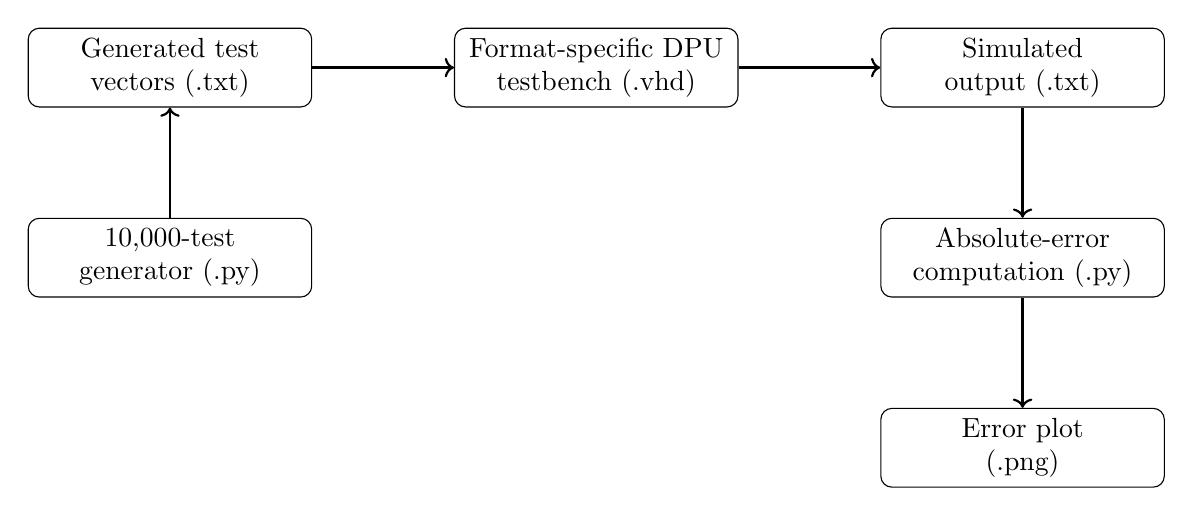
\begin{tikzpicture}[
    node distance=1.4cm and 1.8cm,
    box/.style={
        rectangle,
        draw,
        rounded corners,
        align=center,
        minimum width=3.6cm,
        minimum height=1.0cm
    },
    arrow/.style={->, thick}
]

\node[box] (gen) {10,000-test\\generator (.py)};
\node[box, above=of gen] (txt) {Generated test\\vectors (.txt)};
\node[box, right=of txt] (tb) {Format-specific DPU\\testbench (.vhd)};
\node[box, right=of tb] (out) {Simulated\\output (.txt)};
\node[box, below=of out] (err) {Absolute-error\\computation (.py)};
\node[box, below=of err] (plot) {Error plot\\(.png)};

\draw[arrow] (gen) -- (txt);
\draw[arrow] (txt) -- (tb);
\draw[arrow] (tb) -- (out);
\draw[arrow] (out) -- (err);
\draw[arrow] (err) -- (plot);

\end{tikzpicture}
\caption{Standalone DPU verification flow.}
\label{fig:dpu_standalone_verification_flow}
\end{figure}

More specifically, the initial Python script was used to generate the random test cases and to select the numerical format to be tested. The generated test-vector file contained the input operands and the expected result for each test case. During simulation, the VHDL testbench read these values, applied the inputs to the corresponding DPU, and wrote the simulated output to a separate text file. A Python post-processing script was then used to compare the simulated output against the expected result and compute the absolute error. The resulting error values were finally used to generate validation plots for the different DPU variants, which are presented in the experimental results chapter.


\section{Top-Level Parametric DPU Wrapper}

\section{Validation of the Parametric Wrapper}

\section{Summary}

\chapter{Parametric Tensor Core Unit Architecture}
\label{ch}

\section{Chapter Overview}

The previous chapter introduced the parametric DPU in great details in regards to its implementation. As it has been studied, the constructed parametric DPU computes one dot product operation involving two vectors of four elements each plus an accumulation term. In this chapter, the scope moves one level higher: the goal is to show the design involved in constructing the parametric Tensor Core Unit which uses in its architecture the already described DPU. In fact, the TCU is not just one arithmetic block, but an organized architecture around several DPUs.

The method of RTL design of this upper level unit was built from a bottom-up approach. Several parametric DPUs are grouped inside an octet core. An octet core contains local buffers and the DPU array consisting of the parametric DPUs discussed in the previous chapter. Taking inspiration from NVIDIA, is also known that two octect cores are used inside the TCU datapath. Lastly, a finite state machine has also been designed to control the execution related to the TCU's datapath. 

So this chapter first explains the design objective. Then it introduces the thread-aware execution model. Afterwards it presents the top-level TCU architecture of the first release of designed in the thesis. It also shows the design of the execution related finite state machine. It also describes the datapath organization which will be explained to have the dual-octect structure, buffers and DPU arrays. The chapter also shows how format and width selections are propagated and finally it sumarizes the verification approach related to this unit. This chapter therefore acts as the bridge between the parametric DPU of chapter 3 and the integration work discussed in the following chapters.

\section{Design Objective and Architectural Approach}

As said, the parametric TCU was developed to move from one DPU to larger structure using more then one DPU for treating a larger oriented matrix block. The goal is not only arithmetic hence, but it regards that of organizing several dot-product operations. The TCU in fact is the architectural component which is the layer between the DPU which has been discussed before and the later level involving the processor/GPU integration described in the following chapters of this document.

The goal of the TCU, similarly to the DPU, is to be designed so that it supports more than one number format. This is implictly done already as the unit makes use of the DPU which already supports this. Consequently it is easy to understand that the arithmatic behavior of the TCU changes depending on the selected format/widht just like explained when introducing the parametric DPU.

Finally , from an architectural point of view, the roles of each component forming the TCU are well seperated. This is easily understood as the DPU handles the arithmetic computation specifically. The internal Buffers serve to handle operand staging for reuse mechanisms during the execution. The finite state machine on the other hand serves to handle sequencing. Overall, the datapath of the TCU handles parallel DPU execution. Thanks to this introduced property, it is easier to integrate the design to the modules like GPUs and this will be seen in the later integration related chapters. The next sections remind of the execution model, the top-level wrapper, the finite state machine and datapath and format selection.

\section{Thread-Aware Execution Model}

%paragraph 1: why the thread-awareness matters

The TCU involves operations which are cooperative with each other.  In general the matrix fregments are distributed and organized across multiple threads. Specifically, the concept is that the related hardware is organized considering a groups of threads. This motivates a thread-aware architecture instead of simple standalone arithmetic block \cite{raihan2019modeling}.

%paragraph 2: ThreadGroups and octets Define only what i need. 

Going to more detail, a threadgroup is defined as a group of four threads. In the designed TCU hardware, it is taken into inspiration the fact that two threadgroups cooperate. This specific group of hence eight threads is interprated as an octet. The octet becomes useful because it rapresents a natural unit for feeding part of the tensor core datapath. Also, the octet abstraction has been used conviniently to organize the datapath around groups of eight cooperating lanes. 

%paragraph 3: How this maps to the TCU

In the design of the TCU, the thread-aware idea was very usefull for design inspiration. In fact, it maps to the octect core. One octect core of the TCU corresponds to eight execution lanes / eight threads. The eight lanes are internally divided into two groups of four. Also the scope of the octect core in the design has the scope of the buffers. This means that in the implemented RTL design, the octect core inside the TCU has its own dedicated buffers along with its associated needed DPU array. The purpose is to stage operands and feed multiple parametric DPUs.

%paragraph4 : scope and transition 

This execution model involving the introduced concepts of threadgroups and octects provide the motivation of why it was convinient to build an octet-based design. Essentially, to make the software to hardware map more closer with each other. The following sections describe how this organization has been implemented in the RTL with more focus. First the top level wrapper is introduced and following will be introduced the control finite state machine and the datapath organization descriptions. 

\section{Top-Level Tensor Core Architecture}

The top level TCU is the highest hierarchical component of the overall TCU containing the datapaths as well as the control finite state machine. Externally, it is seen as the whole accelerator block receiving operands and control signals from the outside when it is to be integrated to GPUs or CPUs. The output of its signals are both in terms of control to signal the fact for instance that it is executing, as well as ones related to the data containing the result. The internal complexity of the components is hidden inside this wrapper unit. 

As explained, the wrapper is divided into control path and datapath. the control path is the finite state machine (also referred to as FSM). While the datapath is the computation and operand movement related to the MMA execution. At high level, the datapath consists of two octet cores. And each of these octet core contains buffers and DPU array.  A very high level block diagram initial view of the TCU can hence be visualized in Figure~\ref{fig:tcu_high_level} where the highest level components are observed inside the TCU wrapper.

This organization is the best because it separates nicely the control and datapath and consequently makes the design of the TCU much cleaner and understandable in relation to the threads executing it. It will be seen in more detail in the following sections that the FSM has the duty of deciding the sequence of operations related to a single HMMA instruction to execute on the TCU. While the datapath is the one which performs the staging and the computation itself leading to the final results of the accelerator. The next sections will describe the FSM and the datapath in a much more detailed point of view. 

\begin{figure}[htbp]
\centering
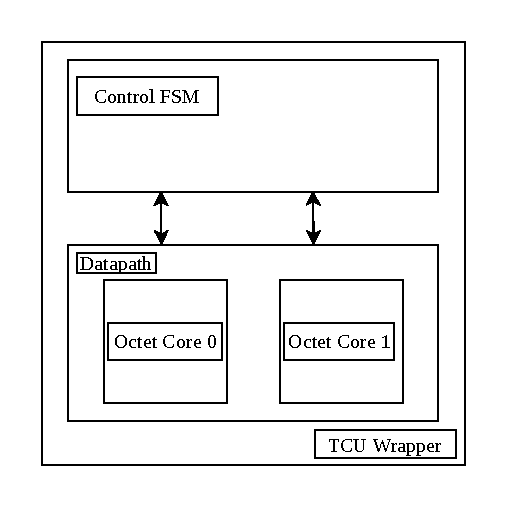
\includegraphics[width=1\textwidth]{Figures/highLevelTCU.pdf}
\caption{High-level organization of the Tensor Core Unit wrapper.}
\label{fig:tcu_high_level}
\end{figure}

\newpage
\section{Control Finite State Machine}

%goal is to introduce the FSM. why it is needed because the TCU operation happens in phases, not all at once.
%idea: fsm is the sequential logic, the datapath is the computational/storage logic.

The parametric TCU that is needed for the matrix workloads cannot do the whole related operation in one single uncontrolled step. In fact, the TCU's execution is performed in an organized matter through a control circuit which consists of a finite state machine guiding the TCU through its HMMA instruction execution. Inspiring from the TCU found in NVIDIA's GPUs, the operands which are related to the matrix multiply and accumulation operations must first load the operands first from their related register files of the threads into the tensor buffers. So, when an HMMA instruction is recognized, the operands must be loaded from the register files of the threads into related buffers.

More specifically, the different operands are loaded in different phases. There is a state dedicated to the fetching of the operands which are related to the A matrix from the register files. In that state, each of the threads which is performing the TCU operation loads into the buffers the associated registers which contain matrix A elements only. Analogously there are also dedicated states for the loading operations of the operands related to the B and C matrices into the related storage buffer elements. Importantly, for the states related to the loading of matrix A , B and C's operands, there are two states for each phase. This is because in the case the operands of the matrices are of 32 bit width, due to the construction of the TCU's buffers which will be introduced later, and due to the limited amount of ports of the register files related to the threads, there need to be two dedicated clock cycles for fetching the four 32 bit elements of a determined operand matrix. Said equivalently, if the load related to the four elements of an operand matrix is within 64 bits in total, then it is possible to fetch the four elements related to a specific matrix in a single clock cycle. Otherwise, the four elements associated to one HMMA instruction can be loaded in the related buffers in two clock cycles, corresponding to traveling in two load states of the FSM instead of one for a specific operand matrix. 

Another design decision of the controller FSM was related to the distinction of the HMMA instruction. In fact HMMA instructions which can execute on the TCU accelerator can be of either'step0' type, or of 'step1' type. If the HMMA instruction is of type step0, then each thread will load the 4 by 4 elements of A, of B and of C related to the operation. Else, if it is of step1 type, the threads need only to load new elements related to the matrix C, as the step1 instructions involve the multiplication of elements of A and B matrices which were loaded by other threads of the same octet which are hence already found in related octet buffers.  

After the loading related steps into the buffers, the datapath executes multiple computation steps which is done through the parametric DPUs. Specifically, in each of the execution steps of the FSM, four parametric DPUs associated to a threadgroup of the octet compute four outputs which correspond to a one by four intermediate result vector of the full four by four final result related to the HMMA instruction. Hence, there need to be in total four states of the FSM to produce the four by four intermediate result matrix associated to the HMMA instruction of a specific thread group. 

Lasty, Figure~\ref{fig:fsm_TCU} shows the concepts of the FSM circuit through the state diagram depiction, showcasing the states described previously and the flow of operations of the HMMA instruction executed on the TCU accelerator. 

\begin{figure}[htbp]
\centering
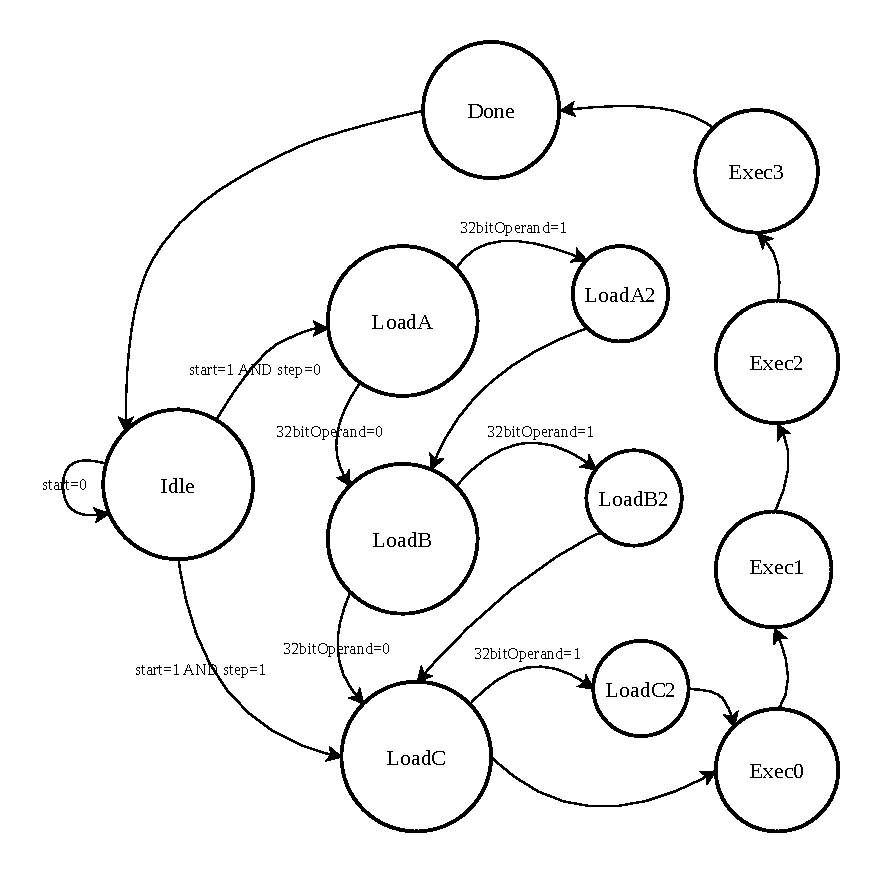
\includegraphics[width=1\textwidth]{Figures/FSM_TCU.pdf}
\caption{First Release of the FSM State Diagram Controlling the TCU's Datapath .}
\label{fig:fsm_TCU}
\end{figure}

\section{Datapath Organization}

%after explaining the control part in the previous section by explaining the fsm, we move to the part related to the computation.
After having explained the FSM circuitry associated to the TCU, which is part of the control related circuitry of the accelerator, it is important to remark the computation related elements composing the TCU. As explained, the FSM decides the sequence of inner steps performed in the related execution of an HMMA instruction done by the threads, while the datapath contains only the hardware descriptions which store the operands related to the singular HMMA instruction and executes the dot products of the MMA operation. As introduced previously, the main organization of the datapath is done by splitting the TCU into two octet cores. Each octet core is associated to two thread groups meaning eight threads in charge of the operability of this inner unit. 

Regarding the components embedded inside an octet core, each octet core contains two general elements: the octet buffers and a parametric DPU array. Both will be analyzed more in detail in this section. The datapath of the TCU in general receives control signals from the FSM and is able to understand on the basis of those signals when to activate the units composing the octet core in order to carry the computation related to the HMMA instruction at hand. Importantly, the datapath propagates related intermediate results and status signals back toward the higher level wrapper TCU unit in order so that eventually they may be  placed inside the related destination registers of the register files. 

\subsection{Dual-Octet Core Structure}

%what is the meaning of organizing the datapath as two octet cores ? ... architectural resons... 
%paragraph1: position in the hiererchy.
Earlier in this document, the top level TCU wrapper has been introduced as an organization of datapath and controller. The datapath part of such organization regarding this implementation can be considered to be non monolithc as it is divided into two symmetric octet core unit components. Each octect core is an intermediate block between the full TCU and the DPU arrays and this is the proof of an hiererchical design.

%paragraph2: meaning of one octect core.
One octet core component specifically groups local computation resources which are shared across two thread groups of four threads each. In fact, in one octet core the values fetched between the two threadgroups composing the octet are shared among them, allowing to efficiently perform the computation by exploiting reusaiblity of associated operands. Therefore this allows to make the overall TCU operation (which is a set of HMMA instructions) to be more efficient since the HMMA instructions related to the 'step1' type previously described have to load less elements into their buffers. This is because certain elements have been already loaded by the threads belonging to a different threadgroup but still related to the same octet. 

The overall high level diagram of the one octet core unit is found in figure Figure~\ref{fig:octetCore}. It shows the buffers associated to the octet of threads which are to utilize such hardware in execution. Specifically, the figure is related to the octet 0 which is the one composed of thred groups 0 and 4. The four threads in thread group 0 utilize lanes 0 to 3 depicted in the picture for loading the related A0, B0, and C0 buffers related to the matrix elements which they are in charge of. While on the other hand, the treads associated to thread group 4 utilize lanes 16 through 19 of the hardware, filling the buffers A1, B1, and C1. In the diagragram it can be noticed that thanks to the buffers, threads can utilize the values loaded by the threads of the opposite thread group of the same octet so that reusability is exploited and efficiency is increased. More details regarding the inner components depicted inside the octet core will be given in the following subsections. 

%paragraph3: why two octet cores
The reason why there are two octet cores is for the increasing of parallelism of the overall accelerator. Also two octet cores keep the datapath symmetric and avoids one large monolithic compuatation block design. Both the cores can be driven by one common control logic. Lastly, two octet cores makes the architecture easier to scale test and also to explain as the mapping of software to hardware is easier to depict.  

\begin{figure}[htbp]
\centering
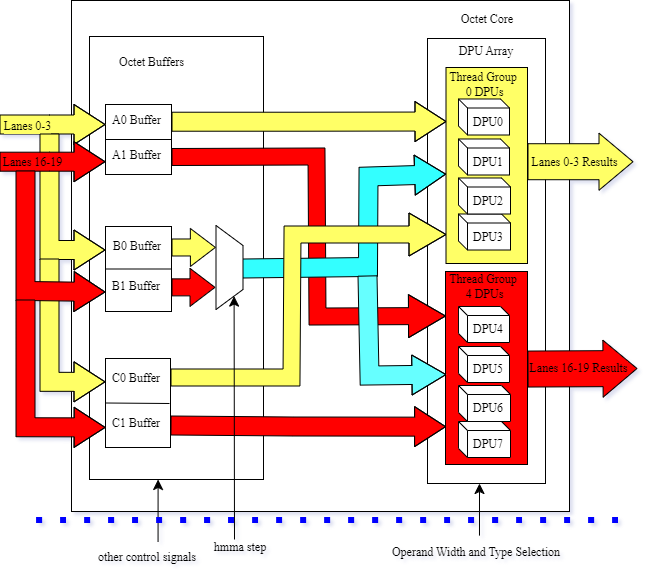
\includegraphics[width=1\textwidth]{Figures/octetCoreRel0.png}
\caption{First Release of the octet Core Datapath Containing the Octet Buffers and the DPU Array Embedded Elements.}
\label{fig:octetCore}
\end{figure}

\newpage
\subsection{Octet Buffers and Operand Staging}

%okay so this section right here will answer... how are operands prepared before the DPU array computes ? 

%paragraph 1: why are buffers needed ?
The buffers are needed for the operand staging fetched from the register files to be utilized in the tensor core's dot product operations. They help because they provide a cleaner execution flow, as well as giving the availability for the threads to utilize operands which were loaded by other threads not belonging to the same thread group of the octet. 

%paragraph 2: what is staged ? 

Buffers related to the octet stage the operands related to 4 by 4 matrix fragments related to the intermediate result calculation of a 4 row by 8 column matrix result. The buffers labeled as A and B in figure are the fragmanents related to matrices A and B while C is the accumulation buffer storing matrix C fragment if the given HMMA instruction belongs to the first set, else it stores the intermediate results needed for accumulation leading to the final result. 

%paragraph 3: FSM control of buffers

To understand which operation to be done by the buffers between loading, or giving the results to the DPU array to execute, the control signal of the FSM are interfaced to the octet buffers. There is a load enable signal which enables the loads synchronously. There is also a specific control signal which selects which kind of buffer needs to be loaded depending on the current state of the FSM, the load phase signal. Additionally, there is the load pair signal for making the buffers execute the loading phase longer in the case the specific format used has operands of 32 bit width. Lastly, as said previously there is the control signal related to making the buffer understnad whether the present HMMA instruction is of step 0 or step 1 type. This last distinguishment is necessary because between step0 and step 1 the four by four HMMA matrix fragment of B utilized for the computation changes in bulk. A detailed rapresentation of the first release of a singular octet buffer is shown in the Figure ~\ref{fig:octetBuffers}. the figure is related to octet 0 again as it mentions lanes 0 to 3 which are ran by the threads of thread group 0 and lanes 16 to 19 which are dedicated to the elements related to thread group 4. Lastly, each of the entries of the buffers loaded by either thread groups stores a one by four vector of a related 4 by 4 matrix fragment.


\begin{figure}[htbp]
\centering
\includegraphics[width=1\textwidth]{Figures/octetBuffer.png}
\caption{First Release of the octet Core Buffers Used For Operand Staging For the DPU Array Execution.}
\label{fig:octetBuffers}
\end{figure}

\newpage
\subsection{Parametric DPU Array}

% trying to answer how are buffered operands actually computed?

In the octet core, after the operands are staged in the buffers they are sent to the computation units which are collected in the DPU array circuit. The DPU array as the name suggests is a collection of parametric DPU units receiving their operands from the buffers. Each DPU of the array performs the dot-product primitive introduced in chapter 3.

Inside the DPU Array there are in total eight DPUs. This means that in parallel, the threads are able to execute eight dot product operations. More in detail, the DPU array of a single octet core outputs two 1 by 4 intermediate resulting vectors which will eventually be staged inside the register files. Considering that the FSM has four execution related states, and considering that the octet core is being executed by two threadgroups in parallel, then in the span of the four FSM execution states two 4 by 4 HMMA result fragments are being computed by the singular octect core.

The DPU array reuses the parametric DPU architecture introduced in chapter 3. For this reason, format and width selection are not redefined at the TCU level. The same selection signals are propagated to the instantiated DPUs, allowing the overall TCU structure to remain unchanged while only the arithmetic behavior inside each DPU changes according to the selected numerical configuration.


From a design point of view, the DPU array related to the octet core is responsible for computing a 4 by 4 intermediate result fragment of the HMMA instruction for each thread group. but since the DPU Array of the octect output two 1x4 vector results per time, there need to be three additional execution steps to give off the remaining six vectors needed for the result of the related HMMA instruction related to the thread groups of the octet. Because of this reason, there are buffers at the output of the array which collect the 1by4 vectors computed by the dpus. This way when the FSM enters a new execution step to calculate a new intermediate resulting 1 by 4 vector contributing to the HMMA fragment result, the previously calculated vector wont be lost. This and the overall DPU array described in this section is shown in the detailed Figure ~\ref{fig:octetDPUArray}. Specifically, the Figure shows the execution when the FSM is in the first of the four execution states the 'exec0' state. The bottom of the figure highlights the overall operation which is being xecuted in the exec0 state by the two threadgroups, as well as the high-level components embedded in one octet DPU array module. 

\begin{figure}[htbp]
\centering
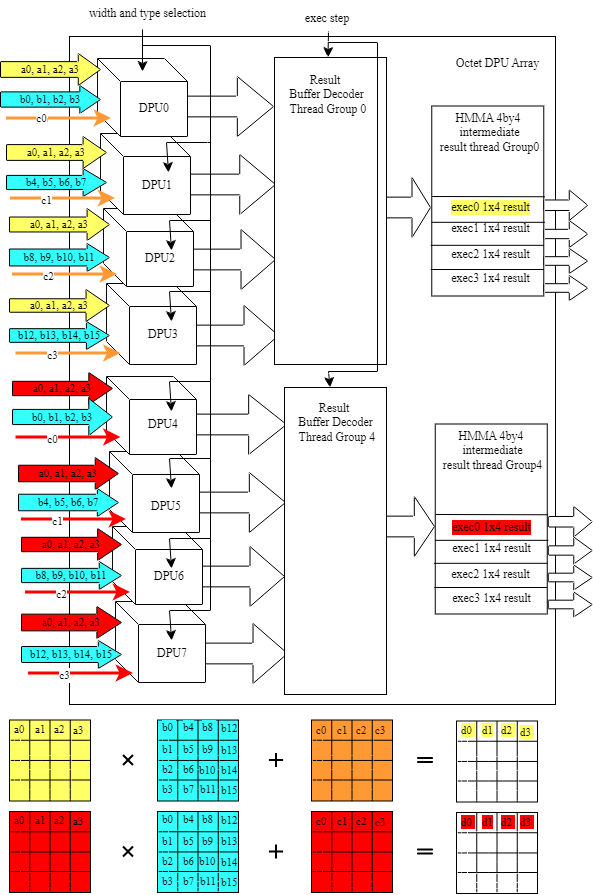
\includegraphics[width=1\textwidth]{Figures/octectDPUArray.png}
\caption{First Release of the octet Core DPU Array and elements involved in the HMMA instruction operation during the 'exec0' FSM state.}
\label{fig:octetDPUArray}
\end{figure}

\newpage
\section{TCU Functional Verification}

%section needed to try and answer: does the standalone TCU execute the intended sequence correctly ? . the goal of this section is to show that the standalone TCU works correctly in simulation.

%paragraph1: the purpose of the verification
The TCU described in the previous sections of this chapter has also been verified through simulation. The overall goal of this step was to check the correct sequence of the standalone TCU. Particularly in checking the correct sequencing of the signals belonging to the FSM and DPU arrays of the octets. The TCU involves two octet core units and hence the verification involves also the correctness of such units implicetly as well. The verification of the standalone TCU accelerator is done at the RTL level simulation level with the Vivado tool.

%paragraph 2: Testbench setup.

For verifying this first release of the parametric TCU, several steps of a general flow have been made. The first step was that of making a python script which was able to produce pseudo-random 16 by 16 A, B and C matrices relating to a multiply accumulation operation which involves four sets of HMMA step 0 and step 1 instructions specifically related to a target format. The python script script outputs the encoded and decoded values of the operands. It also calculates the most accurate decoded and encoded result matrix specific to the test. This first script also produces an input file for the testbench which bacicly gives the elements of the operand matrices so that the buffers are able to obtain the inputs for the tests. Lastly, after the simulation is done, the related RTL-testbench saves the intermediate results of the singular HMMA instructions and most importantly it saves the final 16 by 16 matrix which was obtained by the TCU simulation. Another python script takes this output simulated result and calculates the error with respect to the golden matrix which has been produced by the first script introduced in this flow. 

%paragraph 3: observed simulation behavior. 

To check the correct opration of the implemented inner components of the TCU analyzed in this section, initially the simulation waveforms of Vivado have been observed. After the start is asserted, the FSM follows the expected sequence of operation related specifically to the numerical format which is being tested. More specifically, it was checked if the loading states made the buffers of the accelerators be filled with the values rapresenting the operands. As well as checking if the execution steps happened like intended. Lastly, it was checked visually if the done signal was asserted correctly indicating the end operation of a related HMMA instruction.

%paragraph 4: waveform reference.

An example waveform regarding the simulation of one HMMA step 0 instruction targeting an innter test regarding posit 16 format operands is portrayed inf Figure Figure~\ref{fig:tcu_functional_waveform}. As it can be seen, it portrays the correct flow of the FSM idle, loading, execution and completion related control states. It also presents the content of the octet buffers for the operand matrices being updated in the proper timing, as well as the TCU's signals related to the results for this singular HMMA instruction.

%paragraph 5: 

The waveforms observed in Vivado were particularly useful for debugging the TCU's RTL descriptions if the results of the last HMMA instruction of the full set were different then the expected ones of the final matrix. 


Lastly, it is important to remark that the verification explained in this section only applies to standalone functional RTL behavior. It does not evaluate the area and timing of the associated RTL modules, nor presents the metrics related to the performance and the error of the operations. These specific reults regarding each specific format DPUs embedded inside the TCU will presented in the later chapters of this work. 

\begin{figure}[p]
\centering
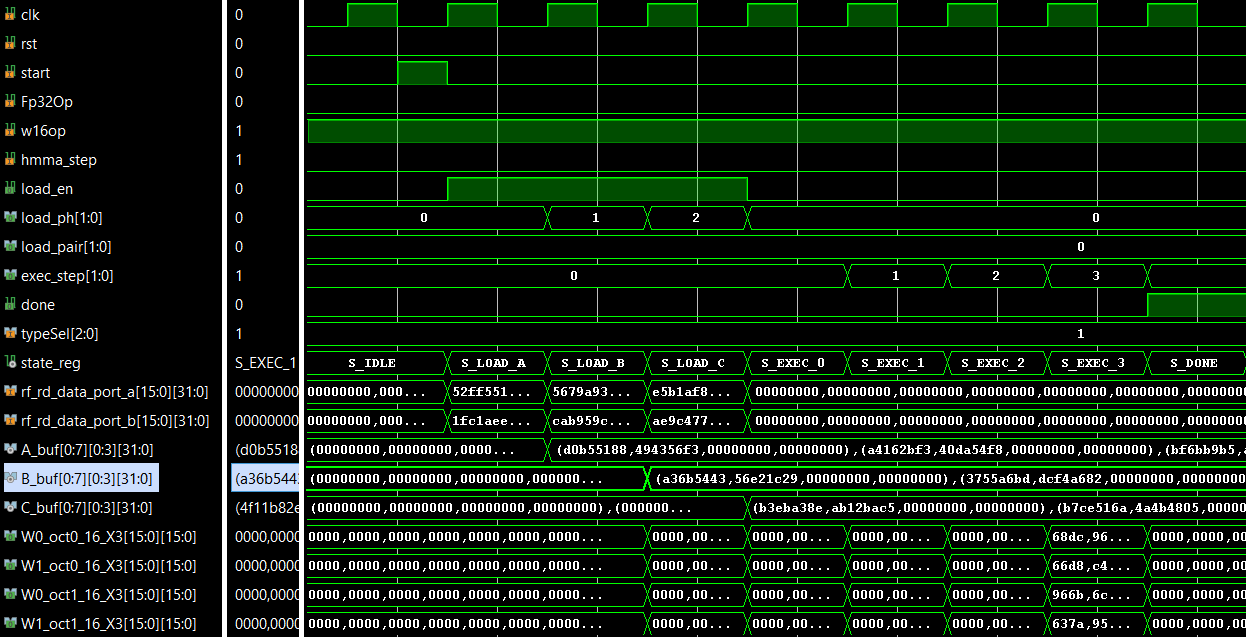
\includegraphics[
    angle=+90,
    width=0.5\textheight
]{Figures/parametricTCUsim.png}
\caption{Standalone RTL simulation waveform of a singular HMMA step 0 instruction in the parametric TCU execution sequence.}
\label{fig:tcu_functional_waveform}
\end{figure}

\newpage
\section{Summary}

This chapter presented in detail the first relase of the parametric TCU architecture. Starting from the concepts introduced related to the granular level parametric DPU introduced in chapter 3, it presented the necessary control and datapath hiererchy needed to implement the parametric higher level accelerator. From a software point of view, it introduced the overall hardware descriptions needed for moving from the singular dot-product operation, to the higher level execution of a matrix multiplication and accumulation operation. 

More in detail, it has been introduced that the higher level wrapper component of the TCU accelerator is split into a FSM and datapath hierechy of design. With the FSM controlling the loading, execution and completion of the singular HMMA related instructions of the sets of the MMA operation, and the datapah organized around two octet cores associated to the 16 threads in total of the SIMD programming model paradigm. Specifically on the datapath, the inner components of the octet core component have been presented : the operand buffers and the DPU array.

Lasty, this chapter presented the functional verification flow that has been done while debugging the components of this first release of the parametric TCU. This debugging has been done through the observation of Vivado waveforms during simulation showing related signals of the components for the related HMMA instructions executed by the testebench of the related formats. 

The next chapters of the thesis will now present the integration step which has been done as soon as the TCU had been varified in its isolated environment. Particularly, chapter 5 will present concepts related to the integration of the TCU component inside a description the Flexgrip plus GPU, and chapter 6 will present the integration of the accelerator with the klessydra T13 RISC-V multi hart core. 

\chapter{FlexGrip Plus Integration of Parametric TCU}

\section{Chapter Overview}

After presenting the parametric TCU in the previous chapter which was verfied independently, the accelerator has been integrated inside the FlexGrip Plus TCU. The goal is to show and prove that the designed parametric TCU becomes usable from GPU execution flow.

This chapter specifically covers the integration related steps needed to insert the RTL description of the TCU inside the RTL description of the FlexGrip Plus GPU. Specifically, it will focus on the changes applied on the existing RTL components which compose the GPU, along with the additional components that are needed for the proper integration. The main design sections of the GPU which has been modified for the integration are the decode stage related logic and the execute stage. The decode logic was modified specifically so that the FlexGrip Plus' programs could recognize custom HMMA instructions supporting the various numerical formats. While the Execute related logic was modified to connect the implemented TCU wrapper itself between the already existing components inside the GPU. The chapter will explain also the Assembly related programs needed in order to prove the functionality of the custom HMMA instruction targeting the accelerator. Lastly, the functional verification flow is also presented in this chapter to show how functional assurance has been achieved when verifying the correct integration of the accelerator into the GPU.

\section{Integration Objective and Warp-Level Mapping}

\section{Custom HMMA Instruction Decode}

\section{Double-TCU Wrapper Integration in the Execute Stage}

\section{Assembly-Level Verification Programs}

\section{Result Collection and Functionall Checking}

\section{Summary}

\chapter{Pulpino Klessydra Core Integration of Parametric TCU}

\section{Chapter Overview}

%paragraph1: start by linking from previous chapters.

The previous chapters presented the standalone first release implementation of the parametric TCU accelerator. Later, the integration of the accelerator into the FlexGrip Plus GPU has also been described. In this new chapter, the focus will be on the intergration of the TCU accelerator inside a open source RTL description of a RISC-V core: the Klessydra T13. The goal of the integration in this environment is to evaluate the TCU's operation in a RISC-V/multi thread core which is a different architecture then a GPU.

%paragraph 2: state the architectural objective.
This chapter will show the design approach applied for the integration to take place. Explaining that a dedicated component branch has been implemented outside the already present instruction execute stage component of the core. Details related to the architecture of such component are provided in a related subsection.

%paragprah 3: Explaining what the chapter will cover.
In the explanation of the integration flow, the concepts related to the construction of custom HMMA instruction the RISC-V core are presented along with what is needed for the decode phase to be able to recognize the custom HMMA instructions. The internal organization of the branch is then analyzed, including instruction capture, operand staging, wrapper control, result capture,
and register-file write-back. 

%paragraph 4: Verification Preview.
Lastly, the chapter disusess the methods utilized to confirm the validation of the integration work. software-level verification progmas and simualtion flow is used to exercise the TCU path and check the produced results by it.

\section{Integration Objective and RISC-V Klessydra T13 Core Context}

%in this section, goal is to explain the context + the objective not yet the detailed RTL.

% goal of the section is to explain why the Klessydra Integration is different from the FlexGrip Plus gpu architecture.

%in this section, the reader should understand what environment im integrating into, Why Klessydra is different target from the FLexGrip Plus, Why the TCU maps naturally to a 16-hart configuration. What the integration objective was. What high-level architectural choice I made.

The integration target focused in this chapter is different then the one described in chapter 5. In fact, the Klessydra T13 RISC-V core is not a GPU inspired architecture like the FLexGrip Plus. More spcifically, unlike the FlexGrip Plus which was a GPU warp oriented architecture containing many cores for thredas to execute in parallel, the Klessydra T13 core is a RISC-V multi-hart core environment. This means that this core is able to execute the program at hand with the help of multiple harts but by using different scheduling mechanisms. Very differently from the GPU, in most cases the harts dont utilize a inner unit all at once in parallel like it was possible in the FLexGrip Plus, but they are scheduled by means of a counter in round robin fashion sequentially. Each of the hart waits its turn to be scheduled in order to occupy a inner execution unit of the core. Hence, the existance of this different topology gives a different validation and integration approach of the TCU inside the core with respect to the integration performed in the FlexGrip Plus. Overall the objective of this integration was to evaluate the parametric TCU in a processor-oriented RISC-V environment rather than only in the GPU-style FLexGrip Plus execution flow.

%paragraph2. Explain the 16-hart/single-wrapper match

In the FLexGrip Plus integration work, the design problem was adapting a 32-thread warp executor to a 16-lane TCU. And like discussed in the previous chapter, this problem had been tackled by constructing a TCU wrapper which contained 2 instances of the parametric TCU. In the Klessydra T13 Core the problem at hand is a bit different. This type of Klessydra Core in fact normally executes at most through the help of 3 harts. However, when building the RTL processor through cmake, the configuration file allows to build the RTL supporting a maximum 16 harts. Hence, in this integration work a single parametric TCU has been instantiated in a Klessydra T13 core with a configuration based on 16 harts.

%paragraph 3: Stating the real integration objective. ---> the objective was not only to instante the TCU. it was to make it usable from the Klessydra pipeline.

The integration objective was not only to instantiate the single instance of the parametric TCU inside Klessydra, but it involved also that to perform additional RTL design work to make the accelerator usable through HMMA instruciton execution. The additional design work involved that of understanding how the core can recognzize the HMMA instruction, in which sections to instantiate the accelerator, additional controls and buffers before of the actual accelerator's execution, and other related decisions.

The starting version of the Klessydra core has inner components arranged so that they follow a four staged pipeline execution involving fetch, decode, execute and write back while executing an instruction. Instead of instantiating the TCU accelerator inside the component related to the instruction execute component, it has been decided to instantiate it as its own seperate branch. Doing so, the TCU component branch receives a request from decode and manages write back and execute separetly.

\section{Custom HMMA Instruction Encoding and Decode Path}


\section{Dedicated TCU Branch Integration in the Processing Pipeline}

\section{Internal Organization of the TCU Branch}

\subsection{Instruction Capture and Format Selection}

\subsection{Operand Collection and Lane Staging}

\subsection{Controller FSM and Tensor-Core Wrapper Execution}

\subsection{Result Capture and Register-File Write-Back}

\section{Software-Level Verification Programs}

\section{Simulation Setup and Functional Verification}

\section{Summary}

\chapter{Experimental Evaluation}

\section{Chapter Overview}

%main message: this chaper moves from architecture and integration to quantitive evaluation.

After the implementation of the architectural parametric DPUs and TCU and the related work regarding the integration of the accelerator inside the FlexGrip Plus and the Klessydra T13 core, an experimental evaluation targeting the accelerator has been performed, and discussed in this chapter.

The Evaluation is done from several point of view: hardware cost, timing/performance, numerical accuracy and resiliency/fault behavior. These qualities are compared among the different numerical formats which are supported in the TCU accelerator. Equivalently this means that the metrics are obtained for the various DPUs inside the TCU. This is because the DPU and its dot-produce/MAC operation is the basic main computational unit used inside the TCU. 

This chapter will portray the results obtain in regards to the metrics mentioned along with providing a detail discussion relating to the obtained numerical results. In the next section, the relative experimental setup is explained for obtaining the metrics regarding the implemented RTL-level descriptions implemented in the thesis.

\section{Experimental Setup}

%purpose of this section is to describe what was evaluated and how. 

As explained in detail in chapter 3, the numerical formats supported in this work for the parametric TCU to handle regard the FP8, FP16, FP32, Posit8, Posit16, Posit32, LNS16, INT8, INT16, FixedPoint8, FixedPoint16 numerical formats. Also, as explained in the background in chapter 2, the TCU accelerator performs the matrix multiply operation thanks to inner parametric DPUs which are implemented with a combination of DPUs each supporting specific numerical formats. In this thesis work it was decided to focus on the DPU level metrics to understand how the different internal DPUs distinguish themselves in terms of hardware area, performance, and resilience. Hence the experimental setup described in this work regards the granular level DPU found inside the TCU accelerator. This decision has been made to decrease the synthesis related and fault resilient timings that are necessary to obtain the results. Henceforth, the results regarding resiliancy performance and synthesi  related to the whole FlexGrip Plus GPU unit with the additional TCU and Klessydra Core unit with its own TCU are to be done in a future work.

Regarding the DPU related tests done for the obtainement of the numerical results regarding the various DPUs, the Vivado Simulation and Synthesis Tools have been utilized. The synthesis tool has been utilized for the calculation of the slack metric related to the singular DPU for the calculation of the performance of DPUs for each of the formats. Furthermore, the synthesis process has also been performed for each of teh DPUs for the objective of obtaining how much gate level area each of teh DPUs for teh formats occupy. During the synthsis of the DPUs, it was decided to use the Vivado synthesis using the AMD/Xilinx Artix-7 FPGA as target device. 

Regarding the results obtained relating to the numerical accuracy and resiliency for each of the DPUs of the formats, the Vivado simulation tool has been utilized confronting the simulated behavior of a specific numerical DPU with respect to the expected one. Both synthesis ans simulation related processes needed for the obtainmnet of the results have been utilized in conjunction with various TCL scripts for launching the synthesis or simulation along also python scripts for the generation of many random tests for the DPU used for example when calculating the numerical accuracy of each target DPU. 

\section{DPU Level Hardware Utilization}

%This section should answer how expensive is each numerical format in hardware.
%how fast is each implementation.
% Which formats are cheaper or heavier and why.

%Paragraph 1: Introducing that each DPU has been synthesised independently.

%Paragraph 2: Explaining the resource metrics and what they mean: LUTs, FFs, DSPs, BRAMs.

For the result obtained regarding the hardware utilization and timing, the synthesis tool has been utilized. Each DPU targeting a different format has been synthesized independently from the others. In regards to the analysis of the area hardware requirement for each of the DPUs, after the synthesis is complete, Vivado generated a resource related report with information regarding the RTL area required and other information. Regarding the area resource metrics, the synthesis report gave for the synthesized DPU at hand information about different area related metrics: 
\begin{itemize} 
    \item  Look Up Tables (LUTs): they are the basic blocks used to implement combinational logic. When the DPU of target in the synthesis needs adders, comparators, multiplexers format decoders and others, the synthesis shows this information through the LUT area metric.
    \item Flip Flops (FFs): sequential storage elements used for registers, pipeline stages and intermediate signals.
    \item (DSP): dedicated arithmetic resources in the FPGA fabric. They are mainly used for the multiplication and multiply-accumulate operation when the synthesis tool maps the target datapth to them.
    \item (BRAM): Block RAMs are dedicated on-chip memory resources. They are mainly used for buffers, memories, and large lookup tables.
\end{itemize}

%Paragraph 3: In-sert the resource utilization table

Table ~\ref{tab:dpu_resource_utilization} summarizes the resource utilization obtained after the synthesis done for each of the synthesized DPU variants. The table confronts the number of LUTs, FFs, DSP blocks and BRAMs required by each numerical format. Since all designs implement the same dot-product operation, the reported values provide a direct comparison of the hardware cost introduced by each arithmetic rapresentation. 

\begin{table}[htbp]
    \centering
    \caption{Post-synthesis resource utilization of the implemented DPU variants.}
    \label{tab:dpu_resource_utilization}
    \begin{tabular}{lrrrr}
        \hline
        \textbf{Format} & \textbf{LUTs} & \textbf{FFs} & \textbf{DSPs} & \textbf{BRAMs} \\
        \hline
        FP8        & 1208 & 80  & 0  & 0 \\
        FP16       & 2015 & 160 & 4  & 0 \\
        FP32       & 4387 & 320 & 8  & 0 \\
        Posit8     & 1430 & 80  & 0  & 0 \\
        Posit16    & 2348 & 160 & 4  & 0 \\
        Posit32    & 5499 & 320 & 16 & 0 \\
        LNS16      & 4917 & 160 & 0  & 0 \\
        FXP8/16    & 424  & 96  & 0  & 0 \\
        FXP16/32   & 1621 & 192 & 0  & 0 \\
        INT8/16    & 363  & 96  & 0  & 0 \\
        INT16/32   & 32   & 64  & 5  & 0 \\
        \hline
    \end{tabular}
\end{table}

%Paragraph 4: Discuss the main trends related to the Resource metrics for the DPUs. discussing in terms of what does the previous table tell the reader ? 

The resource usage changes significantly depending on the format. In general as remarked by the previous table, for the dot product operation regarding the numerical formats with higher bit widths there is more hardware required. For instance as remarked in the table , the LUTs needed for FP32 format are about twice as much then the ones needed for the DPU which targets the FP16 format.  This is effect is shows for all the formats. In fact as observed in the Table, also the posit format is made of DPU which requires more LUT elements when the posit numerical format has widht of 32 bits. The reason for this obtained result is trivial and it is because larger operands require wider embedded adders , multipliers , normalization logic and more internal signals in their respective DPU level hardware organization. 

Another remark which can be made related to the areas of the DPUs regarding the various formats is that the posit formats usually have higher LUT usage than the corresponding floating point formats. In fact for the syntheszed DPUs, the DPU which supports Posit 32 width elements has 1112 LUT elements more with respect to the FP32 synthesized DPU. This is due to the fact that Posit related DPUs involve more additional combinatorial circuits with respect to their floating point counter parts due to the needed regime deocding and the fact that it is a format witch excpects the regime filed of variable length like described in chapter 2. Basically, the Table suggests a trade off with the flexibility and area of implementation since the Posit rapresentation introduces
additional decoding logic. 

Another interesting result displayed by the table regards the LNS16 format compatible DPU. In fact it is seen that this DPU has a number of LUTs which is comparable to the amount of LUTs utilized for the FP32. This indicates how hardware expensive the LNS16 DPU is, as its LUT count is comparable to that of a DPU supporting elements of higher precision. The reason for this negative mismatch is due to the idea that the LNS16 DPU's inner addition modules are more complex then the other embedded addition related to the other formats studied as anticipated in the background chapter 2.

Regarding the DPUs which support the Integer and fixed point formats, their simplestic RTL-description is convayed in the Table as for these formats there are less LUTs required with respect to the formats described previously. Also, interestingly the synthesis tool of Vivado maps very few LUTs for the INT16 related DPU, but this is due to the fact that it maps the synthesized model into an increased count of the DSPs instead.

Regarding the columns regarding the BRAMs, the synthesis tool has mapped 0 BRAMs for each of the DPUs of the formats because they are isolated arithmetic datapaths, not full accelerator subsystems with local memories and buffers. On the other hand for each DPU of each format there is a number of FFs being synthesized because each DPU has included registers for its input operand elements and one register for the result. This was necessary to include for the obtaining of performance related metrics for the DPU which is described more in detail in the next section.

\section{DPU Level Timing Analysis}

%goal of this section is to answer how fast can each DPU implementation run after syntheis ? Which numerical formats create longer critical paths ? Why is that ? 

The timing analysis is equally as important as the resource analysis given in the last section. This is because optimally, the TCU accelerator circuit is integrated inside environments which are almost always synchronous such as the FlexGrip Plus GPU or the Klessydra T13 core which this thesis focused on. So, even though the focus of the thesis gave priority in the functional behavior of the integrated parametric TCU at simulation level, it was still important to provide the performance related metrics of the first relase of the unit to some extend to understand what there is to improve for future versions. Also, this analysis is important to be done at the DPU granular level to find out the differences in the performance related metrics amonf the various implemented DPUs each utilizing a different numerical format of operands. 


%Paragraph 5: Introduce the timing/Fmax metrics and the results data in general.

For styduing the timing analysis and performance between the different DPUs inside the TCU, various related performance metrics have been focused on which are the following ones: 

\begin{itemize}

    \item Critical Path: the longest combinationl path possible between the input registers and result register of a specific synthesized DPU relating to a specific numerical format.
    
    \item Worst Negative Slack (WNS):  the metric portraying whether the design meets the synthesis constraints related to a selected clock frequency. If it is negative, the DPU design does not meet the clock constraints.
    
    \item Estimated Maximum Frequency (Fmax): the approximate maximum clock frequency the design could reach.

\end{itemize}

%Paragraph 6: Insert the main timing trends. 

Just like the hardware resource analysis, the Vivado reports related to timings have been analyzed after the synthesis of each specific numerical format DPU. Also it is important to remark that the synthesis flow used a target clock period of 10 ns. The metrics explained above have been collected from the synthesis timing reports of Vivado for each numerical format and are all gathered in Table~\ref{tab:dpu_timing_results} . The table summarizes the WNS, the estimated critical-path delay and the estimated maximum frequency for all the implemented DPU variants.

\begin{table}[htbp]
    \centering
    \caption{Post-synthesis timing results of the implemented DPU variants.}
    \label{tab:dpu_timing_results}
    \begin{tabular}{lrrr}
        \hline
        \textbf{Format} & \textbf{WNS (ns)} & \textbf{Critical Path (ns)} & \textbf{Estimated Fmax (MHz)} \\
        \hline
        FP8        & -64.029  & 74.029  & 13.51  \\
        FP16       & -95.564  & 105.564 & 9.47   \\
        FP32       & -125.650 & 135.650 & 7.37   \\
        Posit8     & -64.568  & 74.568  & 13.41  \\
        Posit16    & -90.294  & 100.294 & 9.97   \\
        Posit32    & -120.517 & 130.517 & 7.66   \\
        LNS16      & -70.933  & 80.933  & 12.36  \\
        FXP8/16    & -4.365   & 14.365  & 69.61  \\
        FXP16/32   & -9.211   & 19.211  & 52.05  \\
        INT8/16    & 0.516    & 9.484   & 105.44 \\
        INT16/32   & -1.207   & 11.207  & 89.23  \\
        \hline
    \end{tabular}
\end{table}

%paragraph 7: Discuss the main timing trends.

%the goal is to answer what the timing table shows, why some of the formats have lower Fmax with respect to others and what is the important takeAway..

From the previously introduced table, it can be analyzed that out of all the first versions of the DPUs of the numerical formats, only the DPU which takes INT8 related operands respects the imposed clock constraint of 10 ns. Consequently, it makes sense that the similar DPU targeting INT16 operands is almost respecting the constraint with a slack of only -1.206 nanoseconds. The Fixed Point related DPUs are the next fastest DPUs after the integer related DPUs both with a slack less the -10 nanoseconds and are also much faster with respect to the DPUs which target the Posit, the Floating Point and the LNS formats. From the table it can be observed in fact that the Floating Point and Posit formats have much longer critical paths. Specifically the 32 bit variants of these formats are the slowest out of all the othe DPUs and this is because they contain wider datapaths which consequently increase the complexity of the embeeded arithmatic operations  circuits inside the DPU.

Another interesting result is shown when confronting the WNS slack between the Posit8 and FP8 format, the Posit16 and FP16 format, and the Posit32 and FP32 format. When confronting the WNS values between the pairs it can be seen that they are very similar with each other (for instance the Posit 8 DPU has a WNS of -64.568 ns compared to the WNS of -64.029 ns related to the FP8 DPU ). When also considering , as explained in chapter 3, that the floating point DPUs have a different structure (Early Accumulate structure) with respect to the organization of the posit related DPUs (Tree Adder structure), this result shows that independent of the methodology of the DPU design, the critical path delay between these two formats is comparable metric. With regards to the LNS16 DPU, the table proves that it is slower than fixed/integer format DPUs, but comparable to 8 bit posi and floating point ones.

%explaining WHy the results are the ones obtained. discussing a little basically. 

The floating-point and posit implementations show significantly longer critical paths, especially for the 32-bit variants. This can be related to the larger datapath width and to the additional logic required for decoding, alignment, normalization, rounding, or regime handling. LNS16 also shows a relatively long critical path, which is mainly associated with the cost of logarithmic addition and subtraction. 

Since these values are obtained from post-synthesis timing reports, they should be interpreted as comparative estimates rather than final placed-and-routed operating frequencies. Nevertheless, because all DPU variants were evaluated with the same synthesis setup, the results provide a useful indication of the relative timing cost of each numerical format.

\section{Numerical Accuracy Evaluation}

\section{Fault-Injection Methodology}

\section{Fault-Injection Results}

\section{Discussion}

\section{Summary}



\chapter{Discussion}

\section{Precision, Accuracy, and Hardware Complexity}

\section{GPU versus RISC-V Integration Consideration}

\section{Limitation of the Current Release}

\section{Lessons Learned}

\chapter{Conclusion and Future Work}

\section{Summary of Contributions}

\section{Main Findings}

\section{Future Work}


 
\bibliographystyle{unsrt}
\bibliography{biblio}

\end{document}
